\chapter{Behavioural Experiment}
We ran a follow-up experiment to learn more about what information from the EEG data the deep learning neural net used to classify the stimuli. 
First, we investigated whether the vertical red bands from layer 3 (\autoref{fig:model_W}) were associated with a cognitive process that may have supported the neural net's classification, such as recognition of the music. 
Then, we investigated whether the deep learning neural net confused stimuli that were rated as highly similar by humans.
\section{Participants}
Nine participants (four male), aged 22-28, with normal hearing and no history of head injuries took part in this study. 
Six participants had formal music training (2-15 years), and four of those participants played instruments regularly at the time of data collection. 
%On average participants listened attentively to music 1.5 hours per day and had music playing in the background for 3.6 hours per day.
\section{Procedure}
The 12 stimuli were the same songs as those in the original experiment (See \autoref{tab:stimuli_information}).
The experiment had two parts and lasted about 50 mins.
First, participants listened to each of the 12 stimuli and pressed a button when (and if) they recognized the piece of music.
The timing of their key press was recorded. 
During the second part of the experiment, participants were presented with all possible paired combinations of stimuli (78 pairs). 
They listened to the first song followed immediately by the second, and then rated how similar the two songs sounded on a scale from 0 - 100 (0 = the songs sound nothing alike, 100 = the songs sound exactly the same).
Participants were given the following instructions:
\begin{quote}\textit{
Different pieces of music can sound similar or different for many reasons.
For example, different songs may sound similar if sung by the same person, or played on the same instrument.
Other times, the same song might sound very different when sung by different people or played on different instruments.
During this experiment you will hear pairs of songs and rate how similar they sound to you.
You should focus on how generally similar the songs feel to you. Don't worry about whether you are correct or not.}
\end{quote}

\section{Results}
To determine whether the periods of time highlighted by the neural net in layer 3 of \autoref{fig:model_W} (vertical red bands) are related to a cognitive process, such as recognition, we collected the average time at which people recognized these musical pieces (\autoref{fig:RecognitionTime}). 
Based on these results, the highlighted time periods from layer 3 of the neural net were unrelated to the time at which people recognized the piece of music. 
\begin{figure}[h] 
  \begin{center}
%    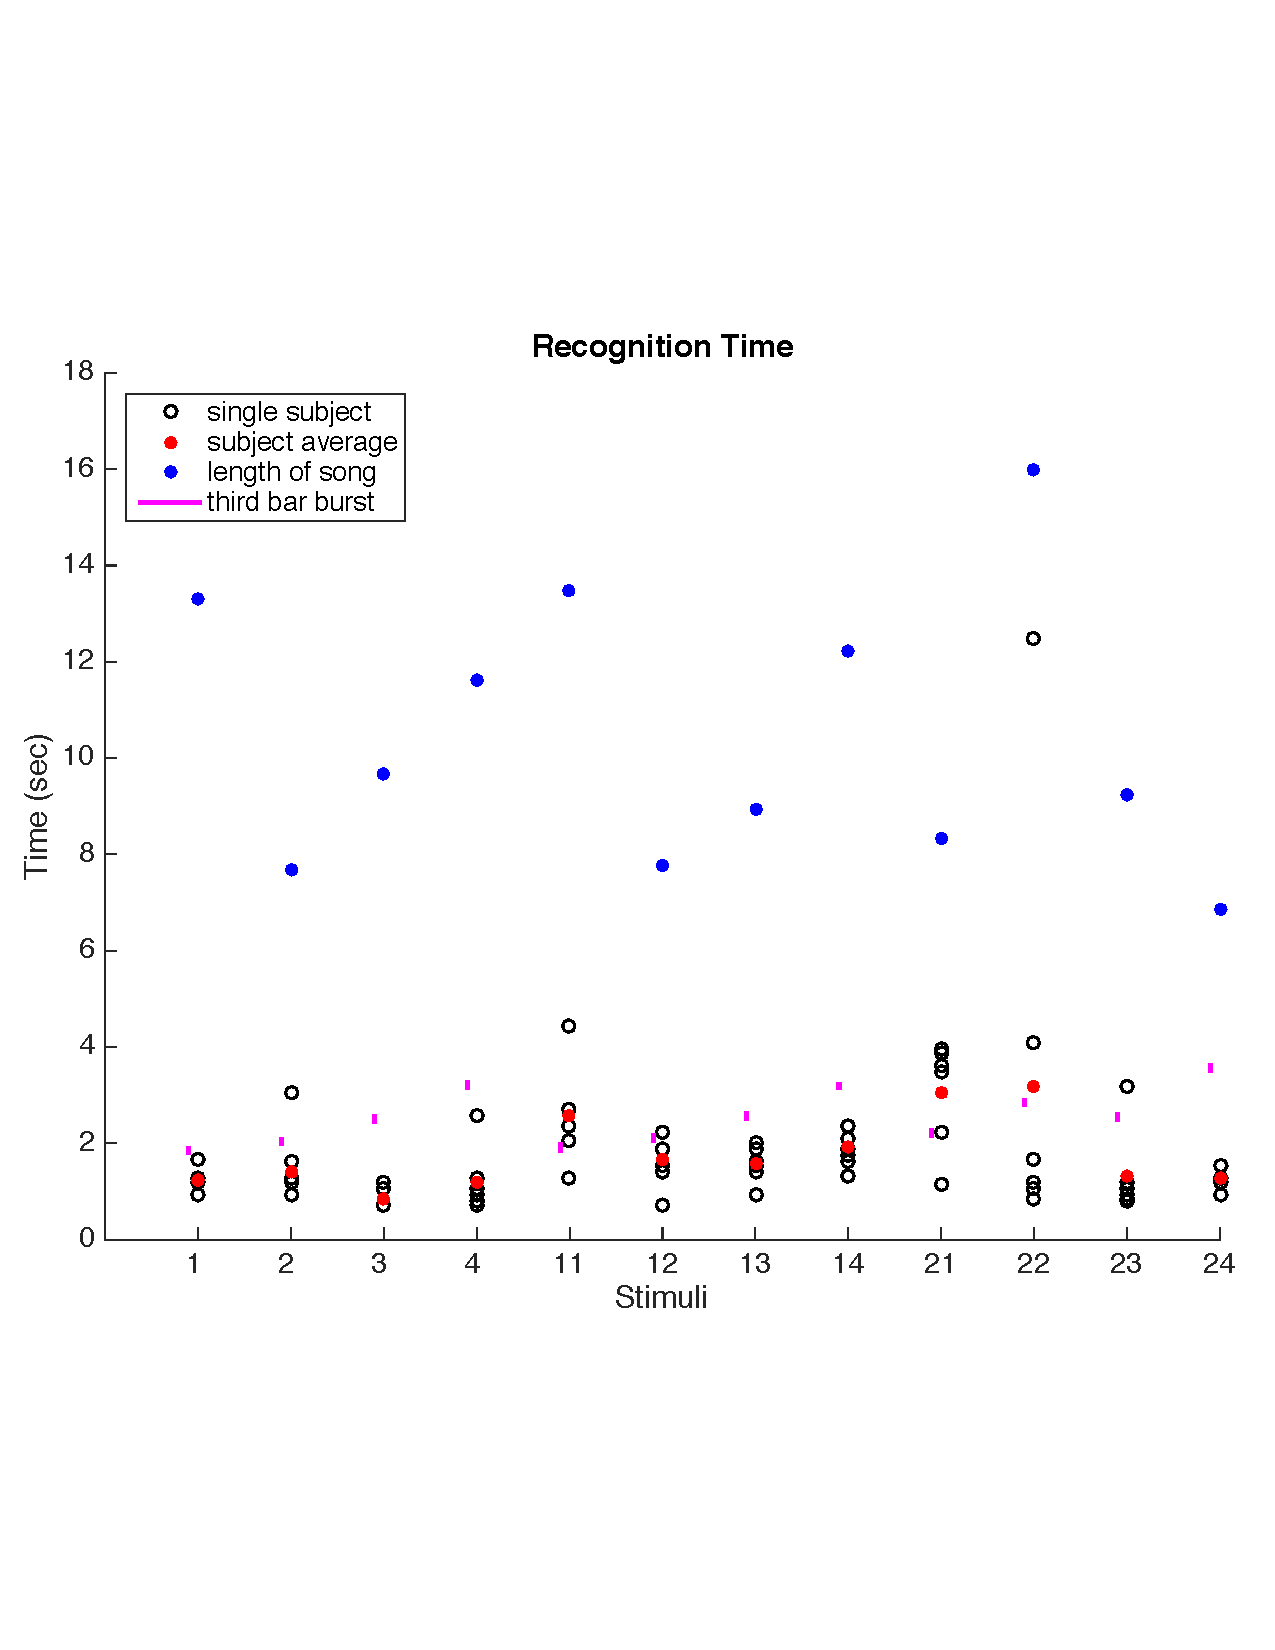
\includegraphics[width=\textwidth,keepaspectratio=true]{Figures/RecognitionTimeGraph}
        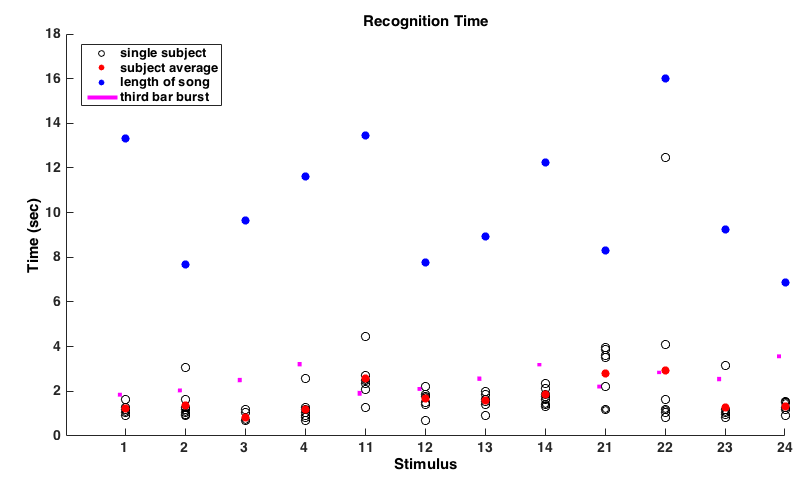
\includegraphics[scale=0.5]{Figures/RecognitionTimeGraph.png}
%   \\\vspace{-0.8em}
    \caption{Average time it takes for participants to recognize these stimuli (red). Individual data is shown in black and song length is shown in blue. The magenta bars indicate the highlighted time periods from layer three in the neural net (\autoref{fig:model_W_confusion}).}
    \label{fig:RecognitionTime}
  \end{center}
%  \vspace{-1em}
\end{figure}

To determine whether the neural net confused songs that humans rated as similar, participants rated pairs of songs on similarity. 
\autoref{fig:Similarity} shows the similarity rating results. 
As expected, participants were nearly perfect at identifying identical songs. 
Lyric/non-lyric pairs of songs were also rated as highly similar, and that is seen in the four, dark squares that are parallel to the diagonal.

The classification accuracy values produced by the neural network in the confusion matrix in \autoref{fig:model_W_binary_confusion} can be interpreted as ``dissimilarity'' scores, so we took their inverse (100 - score) to produce similarity scores, and correlated the similarity matrix with the similarity ratings given by our participants.
The correlation was not significant (r = 0.03, p$>$0.05).
The lack of correlation suggests that the neural network is doing something different from humans when determining similarities between stimuli. 
\begin{figure}[htb] 
  \begin{center}
%    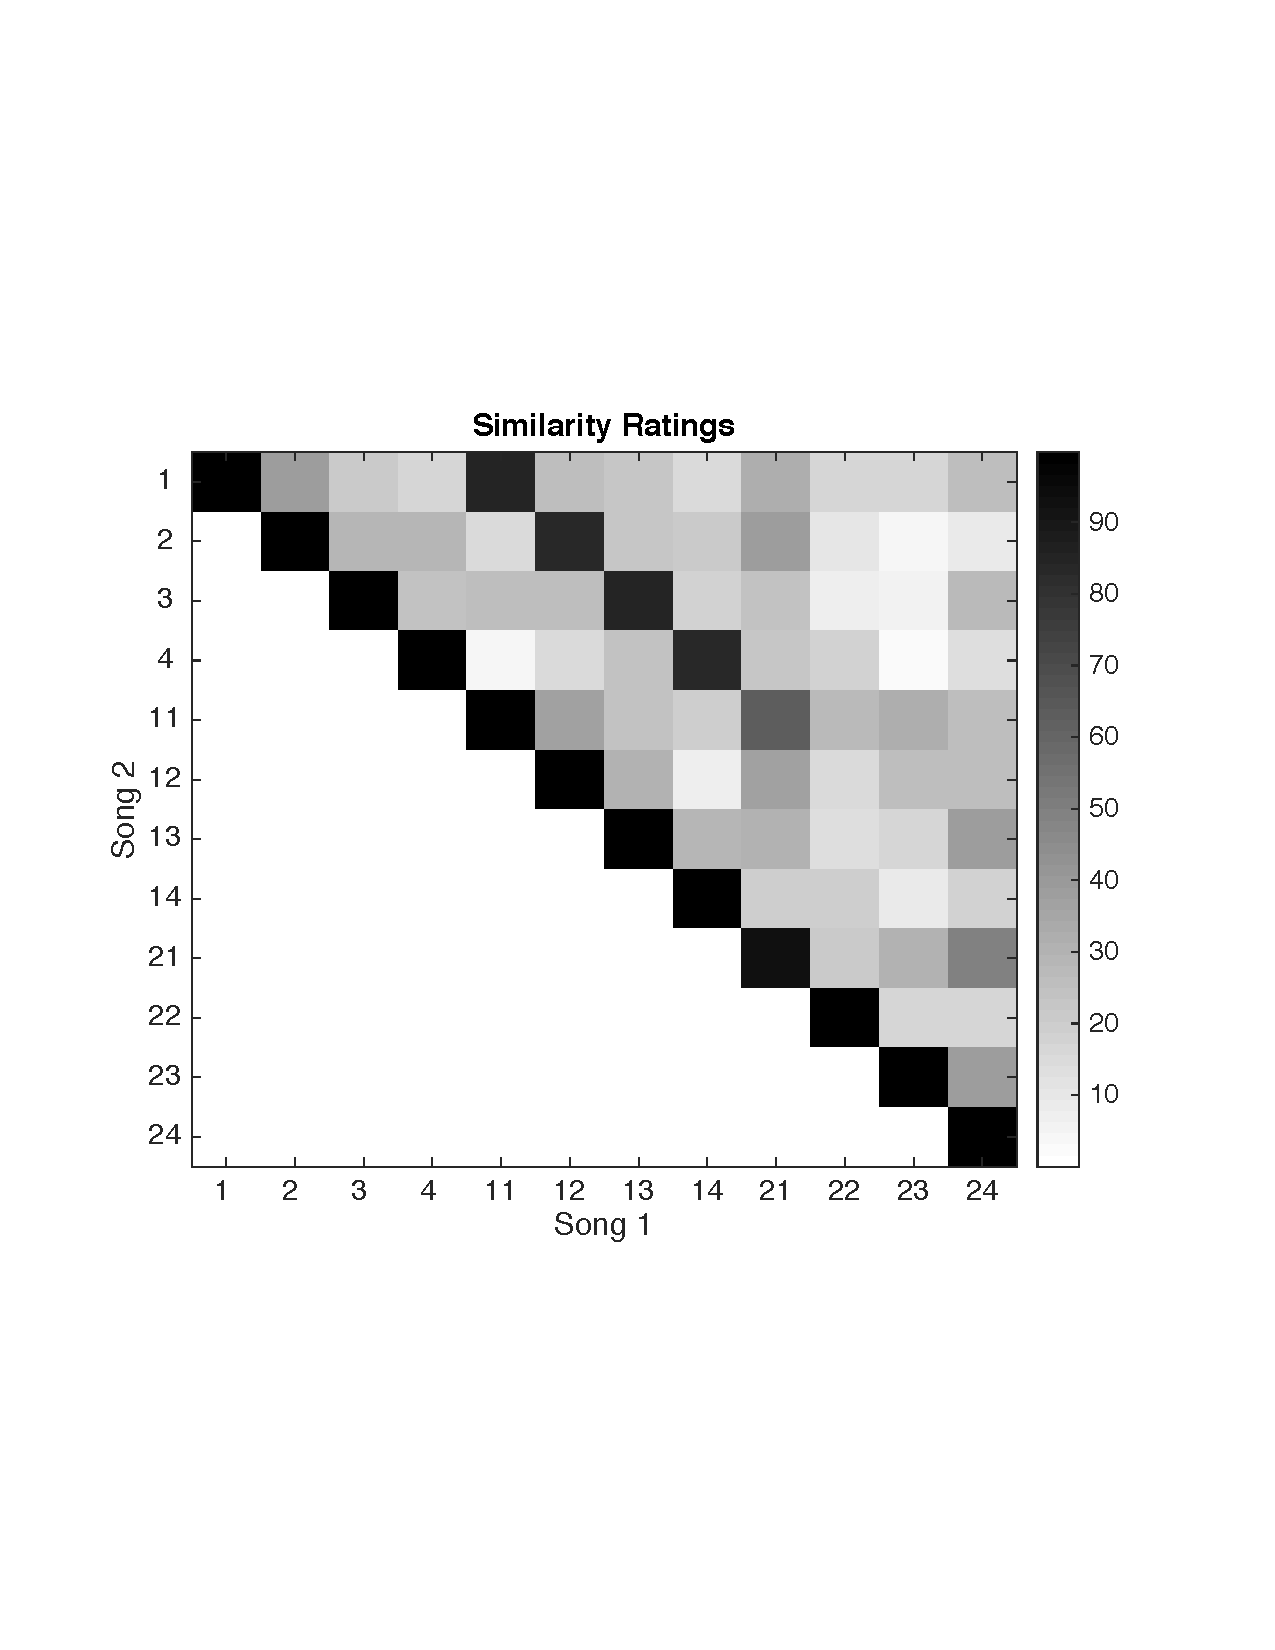
\includegraphics[width=\textwidth,keepaspectratio=true]{Figures/Similarity}
    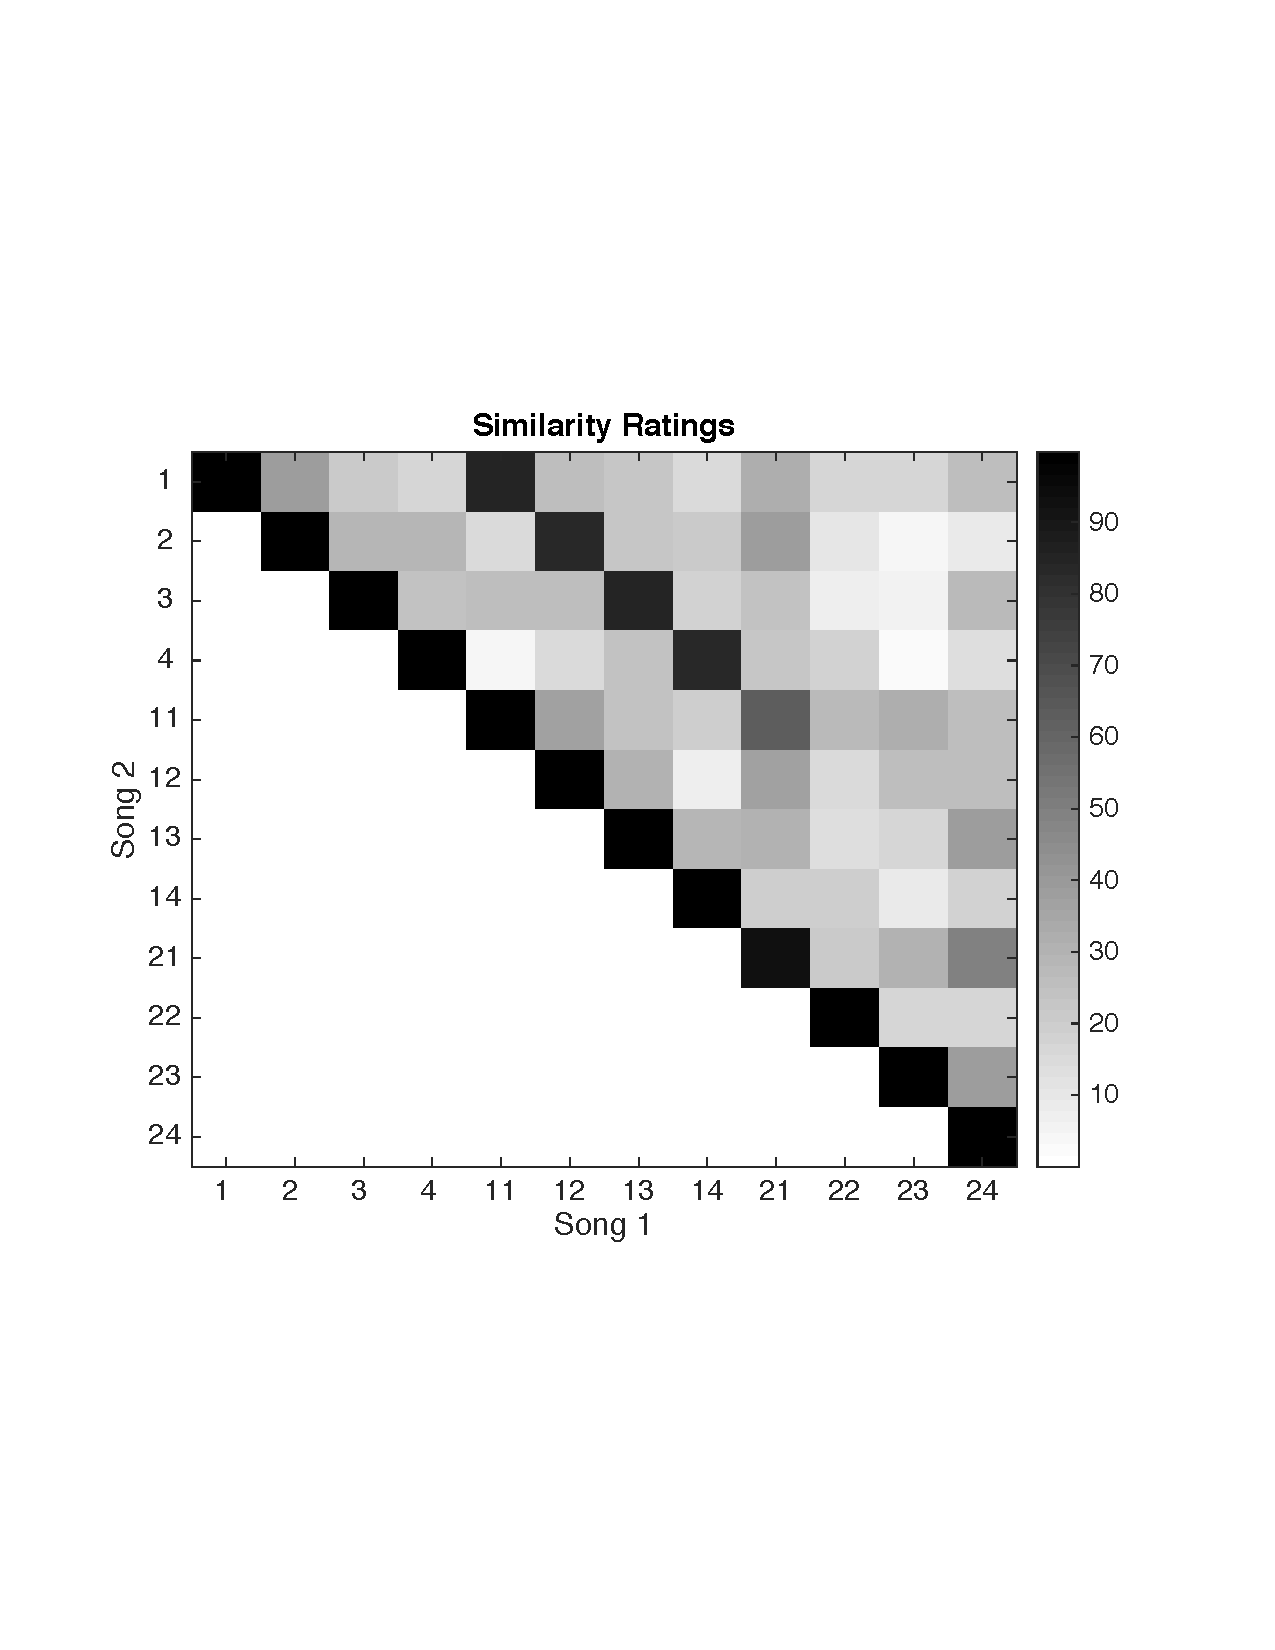
\includegraphics[scale=0.6]{Figures/Similarity}
%   \\\vspace{-0.8em}
    \caption{Similarity ratings (from 0-100) of binary comparisons of all stimuli.}
    \label{fig:Similarity}
  \end{center}
%  \vspace{-1em}
\end{figure}